\startchapter{Socio-Technical Congruence and Failure}
We hypothesize that with the ever growing size of software teams the lack of
effective coordination is the main source of integration failures.  With the
ever growing complexity and sophistication of large software projects,
error-free integrations are not only important but difficult to achieve. The
development work that precedes integrations involves significant coordination of
developers that work in teams and need to rely on the code of others and its
stability. But often code is everything but stable, further contributing to
developers' need to coordinate to keep up with code changes that impact their work. This problem is
amplified in software builds where an entire team needs to integrate their work
and on which the development of new features depends. Not only do
failed builds destabilize the product~\cite{cusumano1997} but they also demotivate
software developers~\cite{holck2004}.

Despite their importance, keeping integrations builds error-free can be a very time consuming
process. A lightweight approach that can determine whether the build contains
failures before invoking the build process is thus very valuable to developers.
This lightweight approach could determine a builds outcome in minutes rather than hours or days. Having a faster way to
assess the quality of a build helps developers to continue working with newest
builds while being aware of its quality. Previous
research~\cite{wolf:icse:2009,hassan:ase:2006} trained predictive models to assess the quality of software builds without the need of invoking large test
suits. Although this research
reaches a high degree of accuracy in their predictions, knowing that a
build will fail does not necessarily help developers to actually prevent
the build from failing.
% limitation of previous research
% SENTENCE HERE ABOUT WHY THIS IS A PROBLEM. SENTENCE ABOUT HOW THIS WAS STUDIED
% BEFORE AND THE LIMITATION THAT RESEARCH HAD ONLY STUDIED PRECTIVE MODELS
% WITHOUT THE ABILITY TO ACT ON THAT KNOWLEDGE.
The goal of this research is to find a way to create actionable knowledge that
developers can act upon to avoid
integration failure.

In this paper we describe a case study of IBM's Jazz project where we leverage
information about socio-technical developer coordination and software builds to
identify pairs of developers that negatively influence the quality of the
upcoming build. Using historical project information we construct socio-technical
networks that capture information about developers with technical dependencies
as well as their ongoing communication as conceptualization of their coordination.
We found that using a support vector machine on a combination of this social
and technical project data yields a powerful predictor of build failure. We
then identify that there are certain pairs of developers that have a
negative influence on the build outcome. On this knowledge developers and management can
act upon to avoid future build failure.

Maintaining proper communication and awareness of work others perform is
important in any kind of project. Specifically in software engineering many studies found
that factors such as geographical and organizational distance have an impact on
communication and even effect software quality~\cite{nagappan:icse:2008}. In our
study we uncover the existence of pairs of
developers, that, if technically dependent in a build but not discussing their
dependencies, have a negative influence on the success on builds. This
actionable knowledge can be integrated in real-time recommender systems that
indicate, based on project historical data, which developer pairs tend to be
failure related. Developers and management can then devise strategies to
prevent the failure before build time. 


The paper is organized as follows: We start with formulating our research
questions (Section~\ref{sec:rq}) followed by putting our research into the
perspective of related work (Section~\ref{sec:relwork}). Section~\ref{sec:data}
covers details about our case study of IBM's Jazz team to investigate
socio-technical coordination in relation to builds. Then
Sections~\ref{sec:prediction} and \ref{sec:pattern} cover the actual analysis and
their discussion. Before we concluding the paper in
Section~\ref{sec:conclusions}, we discuss some practical implications in Section~\ref{sec:implications} and the threats to validity
(Section~\ref{sec:threats}).



%  ONCE SENTENCE HERE REMINDING THE READER THAT IN THIS PAPER WE PROPOSE A
% LIGHTWEIGHT APPROACH THAT LEVERAGES DEVELOPERS SOCIAL NETWORKS BUILT FROM
% PROJECT HISTORICAL DATA AND WHICH IDENTIFIES WHICH DEVELOPER PAIRS ARE
% IMPORTANT WITH RESPECT TO THE QUALITY OF THE UPCOMING BUILD.

\section{Research Questions}
\label{sec:rq}
Communication
is an important mechanism for coordination in software development \cite{curtis:acm:1988,kraut1995:coordination}, especially in maintaining the awareness of changes relevant to your work. Past research showed that a high coverage of technical
dependencies by social relationships correlates with higher productivity of development teams (e.g.~\cite{cataldo:cscw:2006}). 
 We hypothesize that a similar relation
exists between this coverage and the success of software builds. 

Thus
socio-technical networks that capture information about the social and technical
relationships between developers, should predict build failure:

\begin{itemize}
\item[RQ1] Can we use information about relations (technical and social) between
developers to predict build outcome?
\end{itemize}

Although valuable, having a model that predicts build outcome is often not
enough. We seek to generate actionable knowledge upon which developer can act to
avoid a build from failing. Past research suggests that the absence of
communication between developers that are technically dependent leads to
problems, such as slow down in development~\cite{cataldo:esem:2008}.


We hypothesize that due to the high coordination needs the absence of this
important communication also has a negative influence on build outcome. Communication problems can arise from many factors including organizational,
social or technical reasons. Being able to pinpoint
mismatches between technical dependencies and required communication that
relate to build failure is even more important in a team's
ability to devise strategies to avoid build failure. Thus, we
investigate pairs of developers that share a technical dependency without talking
with each other (referred to as \emph{technical pairs}):


\begin{itemize}
\item[RQ2] Are there technical pairs that influence the build outcome?
\end{itemize}

Acknowledging that build failure can be the result
of factors other than lack of developer
communication, e.g. the number of changes or developers in a build~\cite{hassan:ase:2006}, our
analysis also studies the effect of technical pairs in the presence of such
confounding variables. 





%The answer to this question will tell us if we really can devise strategies to
%prevent builds from failing. 


\section{Related Work}
\label{sec:relwork}
Our study aims on integrating work investigating team collaboration and failure prediction to produce actionable knowledge upon which developer can act.
Several studies bear relevance with respect to different dimensions of our work:

\emph{With respect to research on software builds:}
To the best of our knowledge the studies by Hassan et al.~\cite{hassan:ase:2006}
and Wolf et al.~\cite{wolf:icse:2009} are the only studies that conducted
research to predict build outcome. Hassan et al.~\cite{hassan:ase:2006} found
that a combination of social metrics (e.g. number of authors) and technical
metrics (e.g. number of code changes) derived from the source code repository
yield to be best predictor. On the other hand Wolf et al.~\cite{wolf:icse:2009}
solely used metrics that they derived from the social network created from
discussions among developers and showed that communication structure has an
influence on the build outcome.

\emph{With respect to team coordination:}
%Coordination is defined as ``integrating or linking together different parts of
%an organization to accomplish a collective set of tasks''~\cite{vandeven1976}. 
In
order to manage changes and maintain quality, developers must coordinate. In
software development, coordination is largely achieved through communicating with
people who depend on the work that you do \cite{kraut1995:coordination}. The
software engineering literature is recognizing the role of communication as
something that should be nurtured not eliminated and recent
collaborative software development environments aim to support developers'
social interactions along with artifact creation activities~\cite{nakakoji2010:rdc}.

%While a failed build is not necessarily a disaster, it slows down work significantly and is considered extremely undesirable.
%A build result thus serves as an indicator of the health of the software project up until that point in time. If the developers successfully coordinate the integration of code between the previous build and the upcoming build, then the build should succeed.

Ehrlich et al.~\cite{ehrlich:icgse:2006} investgiated how social networks can be
used to leverage knowledge in distributed teams. Backstrom et
al.~\cite{backstrom:kdd:2006} took a more general approach and investigated the
evolution of large social networks and the information they hold. Chung et
al.~\cite{chung:cpr:07} reported in recent work about behavior of individuals
while performing knowledge intensive tasks. There have been a number of studies
that investigated communication structures to identify good
coordination practices
(e.g.~\cite{hinds:cscw:2006,hossain:cscw:2006,bird:fse:2008,hinds:hicss:2008}). In contrast to studies of the general development process, Marczak studied social
networks to identify best practices for requirements management
processes~\cite{marczak:re:2008}.

Inspired by Conways Law~\cite{conway:datamination:1968}, Cataldo et
al.~\cite{cataldo:cscw:2006,cataldo:esem:2008} formulated a coefficient that
measures the alignment of the social and technical networks defining the term of
socio-technical congruence. They observed that higher socio-technical congruence
leads to higher developer
productivity~\cite{cataldo:cscw:2006,cataldo:esem:2008}. Others used this
notion and coefficient to further investigate the effect of congruence
(e.g.~\cite{valetto:msr:2007}). Prior to Cataldo et
al.~\cite{cataldo:cscw:2006,cataldo:esem:2008} proposal,
Ducheneaut~\cite{ducheneaut:cscw:2005} investigated the evolution of social and
technical relationships of open source project participants to see how those
participants become a part of the community.


\emph{With respect to failure prediction:}
There have been a large number of studies looking into predicting failures. For
example, Zimmermann et al.~\cite{zimmermann:icse:2008} used
networks constructed from interdependent binaries to predict the failure
probability of files. They used different metrics characterizing the relationship
binaries have to each other and found that ego centric social network measures
are powerful failure predictors. Previous research conducted at Microsoft used
code complexity metrics, such as cyclomatic complexity or object oriented
metrics, that are derived from source code. Nagappan et
al.~\cite{nagappan:icse:2006} found
that no single source code metric was capable of being a good
predictor over all studied Microsoft projects. Motivated by this study that
suggested that predictions might be domain specific Schr\"oter et
al.~\cite{schroeter:isese:2006} characterized domain of packages in the Eclipse
project by their imports and found them to be a powerful predictor.


\emph{With respect to failures related to team coordination:}
More recent studies started to relate the social with the technical
dimensions of software development to build predictive models. Pinzger et
al.~\cite{pinzger:fse:2008} successfully used social networks connecting
developers via code artifacts to predict failures. Meneely et
al.~\cite{meneely:fse:2008} used similar networks but excluded the code artifacts
and connected the developers directly. Two studies at Microsoft looked into the
geographical~\cite{bird:acm:2009} and organizational~\cite{nagappan:icse:2008}
distance between people that worked on the same binary and the relation to the
failure proneness of said binary. They found that the organizational distance is
a very powerful predictor of failure proneness of binaries whereas the
investigation of geographical distance has little to no effect. A recent
study~\cite{bird:issre:2009} combines the work of Pinzger et
al.~\cite{pinzger:fse:2008} and
Zimmermann~\cite{zimmermann:icse:2008} by creating
socio-technical networks that capture developer contributions and binary
interdependencies. They found this combination to be a more powerful predictor
that works for different software project and even prevails across multiple
revisions of a project.

% talk about the short coming of the failure prediction models
Despite the high predictive power of the state-of-the-art prediction models, most
of them suffer from a profound shortcoming: the knowledge provided by these
models is not always easily actionable. In this work we lie the foundation to
the recommender system described by Schr\"oter et
al.~\cite{schroeter:rsse:2008}. 
%
This recommender system compares social networks derived from technical and social dependencies over successful and failed builds to recommend changing failure related pairs of developers.
%
%AND WHICH\ldots A BIT MORE HERE ABOUT HOW THIS
%RECOMMENDER SYSTEM MAY WORK BASED ON THE RESULTS OF THIS WORK (YOU CAN REPLACE
%THE NEXT SENTENCE WITH THIS DETAIL IF SPACE IS A PROBLEM). 
%
This way we generate knowledge that not only tells us when a build fails but immediately helps us to provide suggestions to prevent the build from failing.





%\pagebreak



\begin{table}[t]
\centering
\begin{tabular}{rrccc}
\toprule
& & Successful & Failed & Total\\
\midrule
&min &1&1&1\\
\#work item & avg  & 16.68&26.52&19.63\\
& max & 111&109&111\\
\midrule
& min & 1&1&1\\
\#change set & avg  & 26.71&46.27&32.57\\
& max & 227&194&227\\
\midrule
& min & 1&1&1\\
\#Developers & avg  & 19.62&28&22.16\\
& max &64&71&71\\
\bottomrule
\end{tabular}
\caption{Statistics on Jazz data: change sets, work items, 
and developers over successful (227), failed (99) and total builds (328).}
\label{tab:jazzbuildinfo}
\end{table}

\begin{figure}[b]
\centering
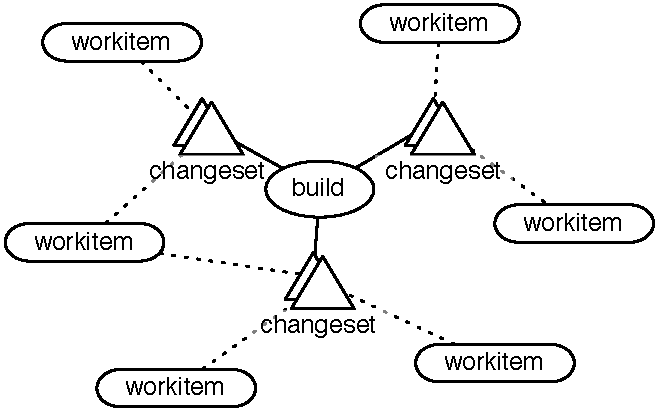
\includegraphics[width=.9\columnwidth]{figures/buildworkitem}
%\vspace{-.3cm}
\caption{Linking work items to builds using change sets.}
\label{fig:buildtowork item}
\end{figure}

\begin{figure}[t]
\centering
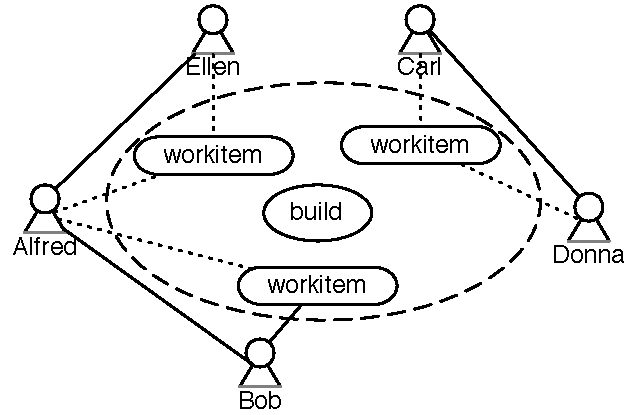
\includegraphics[width=.9\columnwidth]{figures/buildsn}
%\vspace{-.3cm}
\caption{Social network connecting developers through discussions about
work items in a build}
\label{fig:buildsn}
\end{figure}


















\section{Socio-technical coordination\\ and builds in Jazz}
\label{sec:data}
Before we describe our approach to collect data and construct
socio-technical networks in Jazz, we give a brief
description of the Jazz\texttrademark\ team and project. Subsequent,
we explain our approach of mining the project archives to construct
socio-technical networks (Subsections~\ref{subsec:social}
and~\ref{subsec:technical}).

\subsection{Development and Builds in the Jazz Team}
%\subsection{Coordination and integration in Jazz}
The Jazz\tm\ team is a large distributed team and uses the Jazz\tm\ platform for
development. The Jazz\tm\ development involves distributed collaboration over 16
different sites located in the United States, Canada, and Europe. Seven sites are
active in Jazz development and testing. There are 151 active contributors
working in 47 teams at these locations, where developers can belong to multiple
teams. Each team is responsible for developing a subsystem or component of Jazz\tm\.
The team size ranges from 1 to 20 and has an average of 5.7 members. The number
of developers per geographical site ranges from 7 to 24 and is 14.8 in average.

The project uses the \emph{Eclipse Way} development process~\cite{Frost:2007ff}.
It defines six-week iteration cycles, which are separated into planning,
development and stabilization activities. A project management committee
formulates the goals and features for each release at the beginning of the each
iteration, and \emph{work items} represent assignable and traceable tasks for each
team.
Furthermore, the Jazz\texttrademark\ team's development process demands that the developers coordinate using work item discussion. 

The coordination process within
each iteration requires the integration of subsystems developed by individual
Jazz\tm\ teams in a major milestone build of the product.
Each team owns a source code Stream for collaboration and concurrent
implementation of the subsystem. A Stream is the Jazz\tm\ equivalent to a branch of a
source configuration management system, such as Subversion.

A continuous integration process takes place at team-level or project-level. In
frequent intervals, each integration build (referred to a build henceforth)
compiles, packages, and tests the source code of a stream. At the team-level,
contributors commit code changes that are encapsulated in change sets from
their own workspace to the Team Stream. The team integrations build the
subsystem developed by the team. Once a team has a stable version within the Team
Stream, the team publishes the change sets into the Jazz\tm\ Project Integration
Stream. At the project level, the automated
Jazz\tm\ integration builds the subsystems of all teams. 
%The Jazz project-level
%integration takes place \et{nightly}, \et{weekly}, and at the end of each
%iteration -- \et{beta} build.

%%%%%%%%%%%


%We analyze builds created by IBM's Jazz\texttrademark\ development team.
%The Jazz team builds on a regular basis on a nightly and weekly basis.
%Those builds are both on a component and on a project basis.
%
%The Jazz team uses the software they develop the IBM Jazz\texttrademark.
%IBM Jazz\tm\ integrates both source code control and task management.
%Additionally you can also define build schedules as well as general development processes, such as SCRUM.
%
%Thus, the Jazz repository contains all the information from builds over source code changes to tasks, such as bug fixes.
%One advantage of working with he Jazz repository is that links between builds and changes, and changes and tasks are explicit.
%This means we know from the repository which changes contributed to a build and which changes where made to accomplish a task.
%Using this information we can infer which tasks influenced which builds.
%
%The Jazz development team follows the Eclipse Way of development~\cite{Frost:2007ff}.
%The team was between April and July 2008 on a six week development cycle during which a set of features and bug fixes needs to be implemented.
%Instead of extending the cycles when features or bug fixes would take longer to complete they reschedule it for the next cycle.
%
%Another important aspect to their process directly impacts the way they communicate or record their communication.
%Since the Jazz development team is distributed across several sites in North America and Europe they implemented a process that enforces them to record all their communication around any task in the repository.
%This is a best practice implemented by the former Eclipse developer to ensure that people offside do know what's going on and to enable them to contribute.

% some stats about the repository and the team
We mined the Jazz project repository between April and July 2008, and analyzed a
total of 328 builds, out of which 99 were failed and 227 were successful.
Table~\ref{tab:jazzbuildinfo} contains summary statistics describing the Jazz\tm\
repository. We report different aggregations (minimum, average and maximum) of
number of work items, change sets, and developers over all builds. 


%%%%%%%%%%%%%%%%%%%%%%%%%%%%%%%%%%%%%%%%%%%%%%%%%%%%%

%\begin{figure}[t]
%\centering
%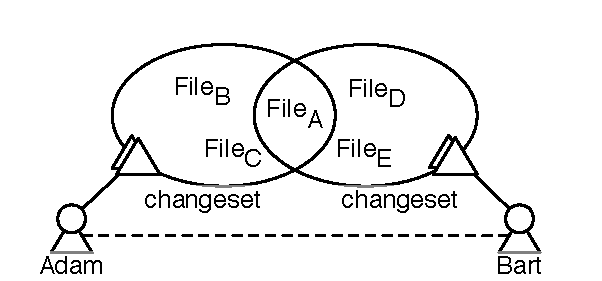
\includegraphics[width=.9\columnwidth]{cochangedfiles}
%%\vspace{-.3cm}
%\caption{Conceptualization of technical relation using co-changed files.}
%\label{fig:technicaldependency}
%\end{figure}

\begin{figure*}[t]
\centering
\subfloat[Identify all change sets related to the social network's build.]{
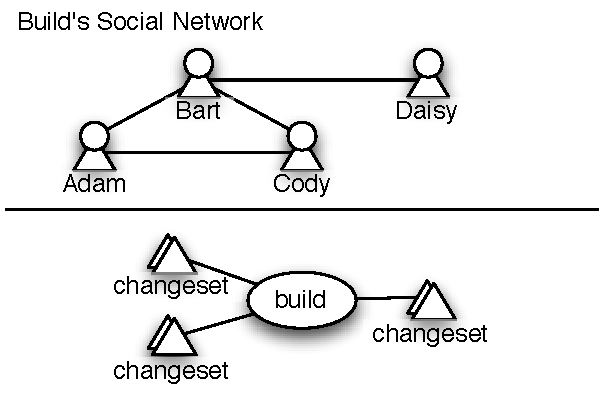
\includegraphics[width=.65\columnwidth]{figures/idcs}
\label{subfig:idcs}
}
\quad
\subfloat[Adding change set owners that are not part of the social network.]{
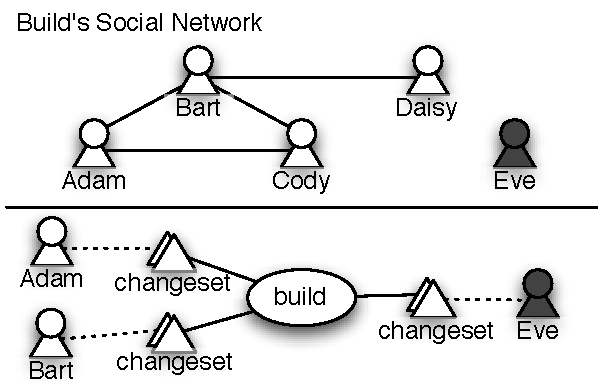
\includegraphics[width=.65\columnwidth]{figures/adduser}
\label{subfig:adduser}
}
\quad
\subfloat[Connect Adam and Bart with a technical edge via the co-changed File$_A$.]{
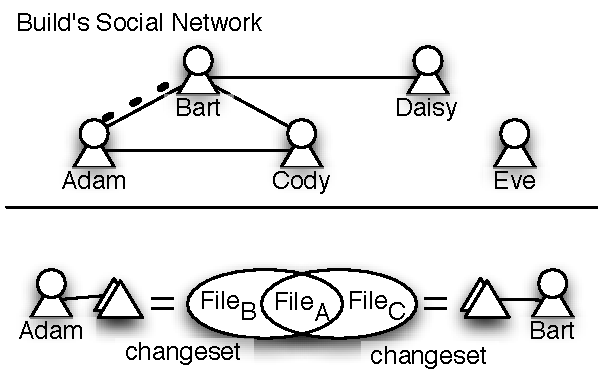
\includegraphics[width=.65\columnwidth]{figures/addedge}
\label{subfig:addedge}
}
%\vspace{-.2cm}
\caption{
Creating a socio-technical network by adding technical dependencies to a build's social-network.}
\label{fig:addtechnicaledge}
\end{figure*}





\subsection{Extracting Social Networks}
\label{subsec:social}
To model the communication between developers for a given build we construct \emph{social networks}. 
We use the information contained in the Jazz\texttrademark\ work items for the construction. 
A \emph{work item} in Jazz\texttrademark\ is the basic unit of work. 
It describes a general task which can be, but is not restricted to, a bug fix or feature request.
Developers coordinate about work on work items by posting comments in a discussion board style which we use as conceptualization of their coordination behavior.
Note that the communication through board discussions is enforced by the team's development process. 


We are interested in constructing a social network for each
build in Jazz\texttrademark. 
To create a social network for a given build we proceed in six steps:

\begin{enumerate}
\item Select the build of interest.
\item Extract change sets that are part of the build.
\item Extract work items linked to the retrieved change sets.
\item Extract developers commenting on a work item before the build's built time.
%\item Retrieve developers that created the retrieved work items.
\item Connect all developers commenting on the same work item.
\end{enumerate}

These steps take us as illustrated in Figure~\ref{fig:buildtowork item}
from a build through a change set to a work item. From the work item we are able to
see who contributed to the work item discussion (Figure~\ref{fig:buildsn}).
These developers become part of the social network and
share a \emph{social edge} if they made a comment on the same work item.
% We use the term \emph{social edge} to describe this connection between two
% developer that commented on the same work item.
Note that all links we use to get from a build to a developer are explicitly contained in
the Jazz\texttrademark\ repository.




\subsection{Constructing Socio-Technical Networks}
\label{subsec:technical}
%\todo{why only change dependencies}
Past research~\cite{nagappan:icse:2005} has shown that dynamic dependencies have the strongest influence on the software quality.
Therefore we use these dynamic dependencies
to construct \emph{socio-technical networks} we use the steps described below
(see Figure~\ref{fig:addtechnicaledge}). We essentially add technical edges to
the build's already constructed social network. In our conceptualization a \emph{technical edge} is a source code
dependency between two developers. A technical dependency between two developers
exists if they changed the same source code file in the build of interest. 

\begin{enumerate}
\item Extract the change sets that are part the build (Figure~\ref{subfig:idcs}).
\item Determine change set owners and add those  that are not already part
of the social network (Figure~\ref{subfig:adduser}).
\item Add a technical edge between change set owners that did change the same file (see Figure~\ref{subfig:addedge}).
\end{enumerate}


We thus call a network that contains both social and technical edges a
\emph{socio-technical network}. The developers in the 
socio-technical network that share both a technical and social edge are said to share
a \emph{socio-technical edge}.











\begin{figure*}[t]
\centering
\subfloat[Evaluation results from the Support Vector Machine.] {
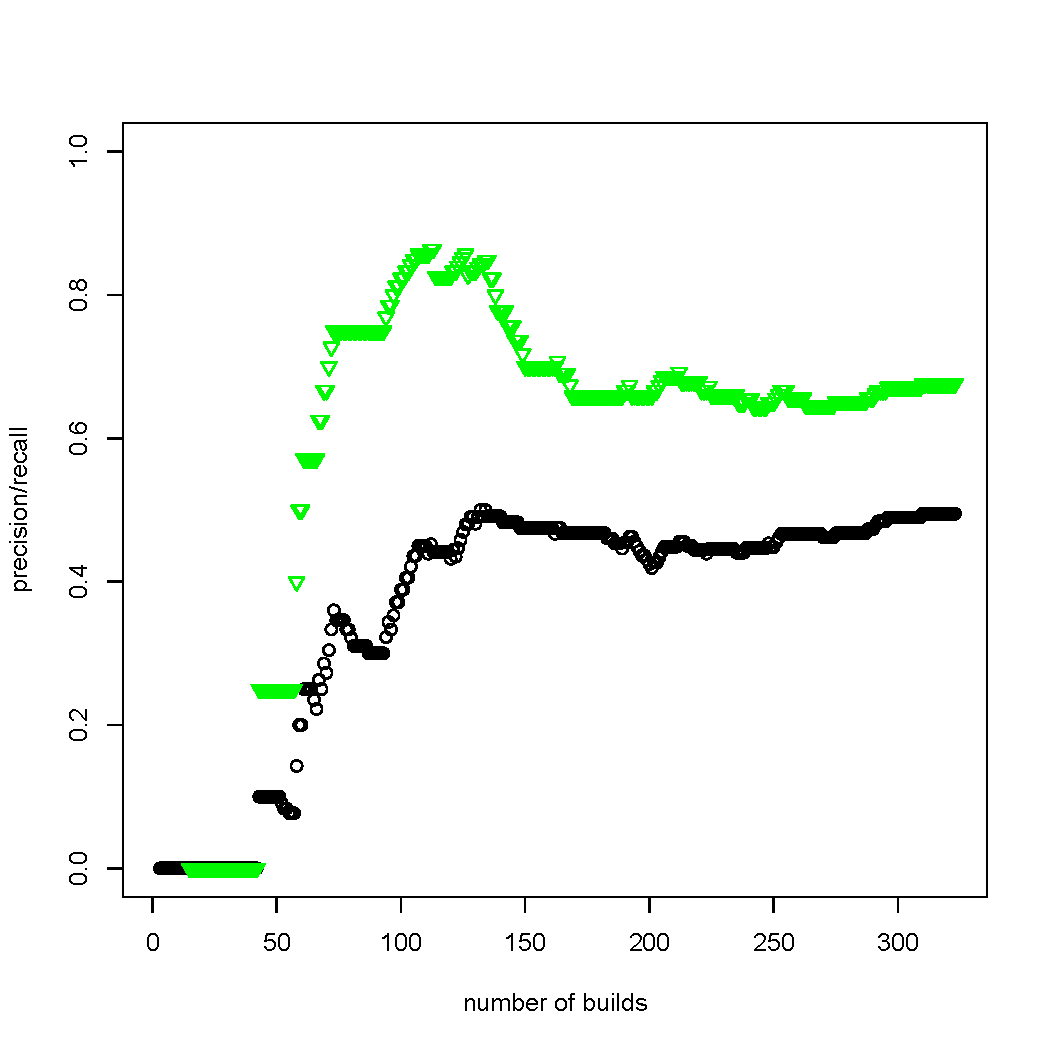
\includegraphics[width=\columnwidth]{figures/precission-recall}
\label{fig:prediction-svm}
}
\subfloat[Evaluation results from the Logistic Regression.] {
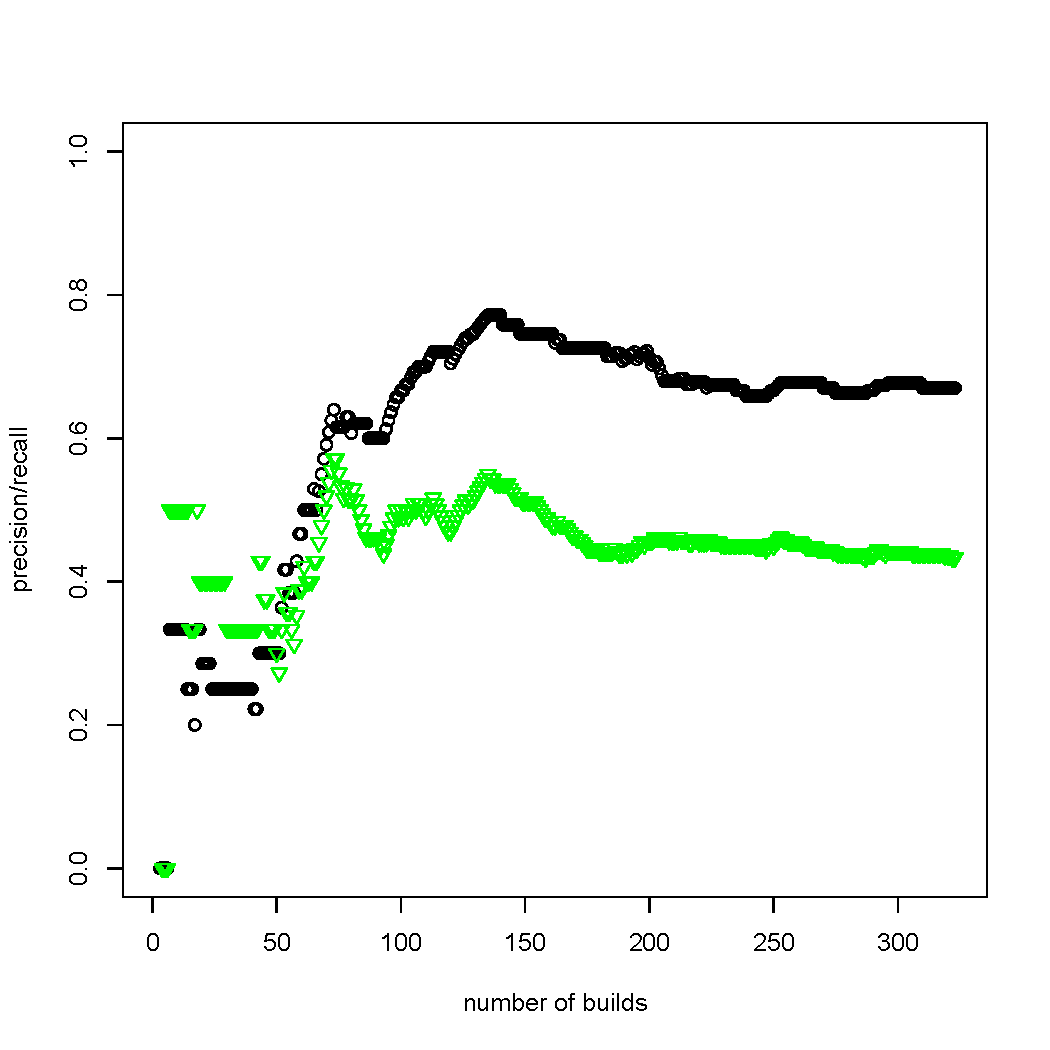
\includegraphics[width=\columnwidth]{figures/precision-recall-logreg}
\label{fig:prediction-logreg}
}
\caption{Plotting the precision (green downward pointing triangles) and recall (black hollow circles) of the support vector machine (left) and the logistic regression (right).}
\label{fig:prediction}
\end{figure*}

\section{Build Failure Prediction}
\label{sec:prediction}
To answer our first research question, we build a predictive model that uses the
constructed socio-technical networks as input to predict whether a build succeeds
or fails. Since we are interested in the practical application of this model we
diverge from the standard evaluation tactic and use a more practical relevant
approach. After we presente the results of our prediction model we discuss their
implications.

\subsection{Model Evaluation}
We train several prediction models, such as logistic regression, support vector
machines, decision trees, and a bayesian classifiers, using features we
extract from the constructed socio-technical networks. Each feature represents a pair of
connected developers in the network and the type of the edge that they are
connected with (i.e. social, technical or socio-technical).

%To evaluate those model, we take a more practical evaluation approach.
To accomplish a more practical evaluation, we order all our social networks by the time the build they were constructed from was tested.
Having the networks ordered according to build time we evaluate our prediction model in the following five steps:%\todo{make pictures}

\begin{enumerate}
\item Get the first $n$ networks and perform a principle component analysis on the extracted features.
\item Select the principal components that explain the most variance until 95\% of the total variance of the training set can be explained.
%\item Determine the principal components of the first $n$ networks.
\item Train the model using the principal components of the first $n$ networks.
\item Test the model on network $n+1$ after transforming it to the determined principal components.
\item Increase $n$ by 1 and repeat until $n+1$ is the size of complete data set.
\end{enumerate}

This evaluation technique is meant to simulate the actual usage of the prediction model.
In software practice builds come in one by one.
This means that whenever a build has been verified the model can be extended using the social network from the newest build for training. 
This method of evaluation is closer to the actual usage in the field than
random splits or cross validation.

We used two coefficients to assess the models quality at any given time: recall (Eq.~\ref{eq:recall}) and precision (Eq.~\ref{eq:precision}).
The recall of a model describes the percentage of how many failed builds where predicted correctly.
This translates into the formula:

\begin{equation}
\label{eq:recall}
\text{recall}=\frac{\text{Correctly \emph{as failed} Predicted Builds}}{\text{All Failed Builds}}
\end{equation}

Precision on the other hand describes the percentage of how many of the \emph{as failed} predicted builds are actually failed builds. Thus we can express precision using the following formula:

\begin{equation}
\label{eq:precision}
\text{precision}=\frac{\text{Correctly \emph{as failed} Predicted Builds}}{\text{All \emph{as failed} Predicted Builds}}
\end{equation}

Both recall and precision lie in the interval from 0 to 1, with 1 being best and 0 being worst.
We compute the recall and precision for each iteration by accumulating the prediction results of all previous prediction results.
For example if we went through 20 iterations we create a contingency table from the predicted results for the last 20 builds.
Each prediction can have one of four outcomes: (1) correctly predicted \emph{as failed}, (2) correctly predicted as succeeded, (3) falsely predicted \emph{as failed}, and (4) falsely predicted as succeeded.
Adding those numbers till the most recent prediction enables us to compute precision and recall.


The current standard evaluation for failure prediction models in software engineering is to take the data set and generate a number of random splits (e.g.~\cite{zimmermann:icse:2008,schroeter:isese:2006,nagappan:icse:2008}).
A random split partitions the data into a training and a testing data set, where the model is trained with the training data and then evaluated using the testing set.
Other also used cross validation which creates $n$ partitions and tests with each partition while training with the remaining $n-1$ partitions (e.g.~\cite{wolf:icse:2009}).

Although random splits and cross validation allow for a random combination, they completely ignore the explicit order.
This leads to the problem that random splits and cross validation allow features that might emerge later and should not have been available to be used for training.
For example, if a developer joins the project after it started, she cannot have been present in any of the networks previous to her date of joining the project.
This means that the model at first cannot use any information about her connections to others.

%%%%%%%%%%%%%%%%%%%%%%%%%%%%%%%



\subsection{Results}
Of the prediction models we evaluated, we present the results for the support
vector machine and the logistical regression. The support vector machine produced
the best results whereas the logistical regression serves as comparison to the
support vector machine results as well as indicating the reliability of
the regression analysis presented later in Section~\ref{sec:pattern}.

% describe support vector machine \todo{talk about three sections of the figures}
Figure~\ref{fig:prediction} shows the recall and precision values for the
suport vector machine and the logistical regression models. The green downward
pointing triangles represent the precision of the model for each iteration, note that we started training each model with at least three data points. The black circles represent the recall of a model for each
iteration.

Both Subfigures in Figure~\ref{fig:prediction} can be divided into three
sections. The first section is comprised of the first 70-80 iterations where,
by a manual investigation, we observe that the support vector machine predicts almost everything to be successful in contrast to the unstable logistic regression.

The middle section is characterized by a peek efficiency between 100 and 150
iterations in both prediction models. Before that peak both models underperform, where the support vector machine suffers more than the logistic regression from a small data set.

In the last segment after 150-180 iteration the precision and recall values
stabilize over both models. In contrast to the logistic regression the support vector machine obtains a higher precision and a lower recall with a slight upward trend.
The support vector machine ended with a precision of $.68$ (median: $.67$) and a recall of $.49$ (median: $.45$) whereas the logistic regression obtained a precision and recall value of $.43$ (median: $.45$) and $.67$ (median: $.67$) respectively.












\subsection{Discussion}
% - why did we fulfill our objective
Although the overall performance of the models is not yet practical due to low
precision and recall, these results are interesting. On the one hand, we consider
answering our first research question with yes: we can use developer pairs to
predict build failure. We consider the model to be sufficient because we, as Wolf
et al.~\cite{wolf:icse:2009}, outperform a random guess which would have
resulted in both recall and precision of less than $.33$, which is the percentage of failed
builds. To our knowledge there have been only two studies that focused on
predicting build outcomes: by Hassan et al.~\cite{hassan:ase:2006} and by Wolf et
al.~\cite{wolf:icse:2009}. Our approach places itself between the results of both
studies with our study being better than results obtained by Wolf et
al.~\cite{wolf:icse:2009} but being worse than Hassans et
al.~\cite{hassan:ase:2006} approach.

Despite of outperforming the random guess the precision of our models is of concern because
it indicates the rate at which we falsely report a build to fail. With a median
 precision of $.67$, every third of the \emph{as failed} build predicted by the support
 vector machine would be a false positive. Besides the low trust a developer
 can develop in the model, it also reports less than half of the failed builds
 as failed.


% - why is the beginning so weak
We provide some possible explanations here. In the first part of the
Figures~\ref{fig:prediction-svm} and~\ref{fig:prediction-logreg}, we observed
that all models perform poorly as long as they have less than 100 builds to train
on. After investigating the first 100 builds we found that new
developers are continually appearing in the development pairs. This means that
prediction models need to make predictions without having enough knowledge to
train on, thus resorting to predict the build to be the most likely outcome, to be OK.

%- check peeks with respect to new developers entering the team
A peak in the interval of 100-150 iterations occurred in both models for both recall and precision.
Within this interval the team changed and new people joined the project and people where reallocated to work on new functionality which meant creating new dependencies and leaving old dependencies behind.
This change in dependencies confused the model in a way that it did not perform as well.
Both models stabilize over time with the support vector machine exhibiting a slight upward trend.

% - what is the next step
Since the goal of this research is to find a way to create actionable knowledge
to avoid build failure, building a prediction model was the first step to show
that developer pairs have an effect on the actual prediction. The results from
the prediction models is first evidence that developer relationships have an
influence on the build. Next we continue with perusing our second research
question that examined the relationship between particular developer
pairs (i.e. technical pairs) and build results. This will help us
investigate how we might prevent builds from failing by changing the
nature of developer relations in these pairs.





\begin{table}[t]
\centering%\vspace{1cm}
\begin{tabular}{rcc}
\toprule
 & successful & failed  \\
 \midrule
(Adam, Bart) & 3 & 13 \\
$\neg$ (Adam, Bart) & 224 & 86\\
\midrule
total&227&99\\\bottomrule
%User3493, User2943 & 3 & 13
\end{tabular}
\caption{Contingency table for technical pair (Adam, Bart) in relation to build
success or failure}
\label{tab:contingencytable}
\end{table}



\addtocounter{table}{1}
\begin{table*}[t]
\centering
\subfloat[Twenty most frequent \emph{technical pairs} that are failure-related.]{
\begin{tabular}{@{\hspace{.2cm}}ccc@{\hspace{.75cm}}c@{\hspace{.2cm}}}
\toprule
Pair & \#successful & \#failed & $p_x$\\
\midrule
%Cody-Daisy&  0 & 12 & 1.0000 \\
%Adam-Ina & 0 & \phantom{1}8 & 1.0000 \\
%Adam-Kim& 0 & \phantom{1}8 & 1.0000 \\
%Adam-Nina & 0 & \phantom{1}6 & 1.0000 \\
%Fred-Gina& 0 & \phantom{1}6 & 1.0000 \\
%Gina-Oliver & 0 & \phantom{1}6 & 1.0000 \\
%Adam-Daisy& 1 & 14 & 0.9720\\%67 \\
%Bart-Daisy& 1 & \phantom{1}9 & 0.9572\\%127 \\
%Adam-Lisa& 1 & \phantom{1}8 & 0.9521\\%204 \\
%Bart-Eve & 2 & 11 & 0.9318\\%403 \\
%\textbf{Adam}-\textbf{Bart}& \textbf{3} & \textbf{13} & \textbf{0.9150}\\%485 \\
%Bart-Cody & 3 & 13 & 0.9150\\%485 \\
%Adam-Eve & 4 & 16 & 0.9086\\%162 \\
%Daisy-Ina & 3 & 12 & 0.9086\\%162 \\
%Cody-Fred& 3 & 10 & 0.8923\\%077 \\
%Bart-Herb & 3 & 10 & 0.8923\\%077 \\
%Cody-Eve & 5 & 15 & 0.8817\\%568 \\
%Adam-Jim & 4 & 11 & 0.8723\\%792 \\
%Herb-Paul & 5 & 12 & 0.8564\\%397 \\
%Mike-Rob& 6 & 13 & 0.8434\\%004\\
%Adam-Fred & 6 & 13 & 0.8434\\%004\\
%
%User11137, User4105 & 0 & 12 & 1.0000 \\
%User2943, User13877 & 0 & 8 & 1.0000 \\
%User7438, User2943 & 0 & 8 & 1.0000 \\
%User2943, User2810 & 0 & 6 & 1.0000 \\
%User8645, User1976 & 0 & 6 & 1.0000 \\
%User8645, User2267 & 0 & 6 & 1.0000 \\
%User11137, User2943 & 1 & 14 & 0.9675\\%908 \\
%User11137, User3493 & 1 & 9 & 0.9504\\%773 \\
%User6012, User2943 & 1 & 8 & 0.9446\\%298 \\
%User3493, User2435 & 2 & 11 & 0.9214\\%387 \\
%User3493, User2943 & 3 & 13 & 0.9023\\%53 \\
%User3493, User4105 & 3 & 13 & 0.9023\\%53 \\
%User2943, User2435 & 4 & 16 & 0.8950\\%695 \\
%User11137, User13877 & 3 & 12 & 0.8950\\%695 \\
%User1976, User4105 & 3 & 10 & 0.8766\\%716 \\
%User3493, User6339 & 3 & 10 & 0.8766\\%716 \\
%User4105, User2435 & 5 & 15 & 0.8648\\%208 \\
%User2943, User9017 & 4 & 11 & 0.8543\\%22 \\
%User6339, User13875 & 5 & 12 & 0.8365\\%498 \\
%User10979, User3385 & 6 & 13 & 0.8220\\%793\\
%User2943, User1976 & 6 & 13 & 0.8220\\%793 \\
%
(Cody, Daisy)	&	0&	12&	1		\\ %user11137.user4105.T
(Adam, Daisy)	&	1&	14&	0.9697	\\ %user11137.user2943.T
(Bart, Eve)	&	2&	11&	0.9265	\\ %user3493.user2435.T
(Adam, Bart)	&	3&	13&	0.9085	\\ %user3493.user2943.T
(Bart, Cody)	&	3&	13&	0.9085	\\ %user3493.user4105.T
(Adam, Eve)	&	4&	16&	0.9016	\\ %user2943.user2435.T
(Daisy, Ina)	&	3&	12&	0.9016	\\ %user11137.user13877.T
(Cody, Fred)	&	3&	10&	0.8843	\\ %user1976.user4105.T
(Bart, Herb)	&	3&	10&	0.8843	\\ %user3493.user6339.T
(Cody, Eve)	&	5&	15&	0.8730	\\ %user4105.user2435.T
(Adam, Jim)	&	4&	11&	0.8631	\\ %user2943.user9017.T
(Herb, Paul)	&	5&	12&	0.8462	\\ %user6339.user13875.T
(Cody, Fred)	&	5&	11&	0.8345	\\ %user11137.user1976.T
(Mike, Rob)	&	6&	13&	0.8324	\\ %user10979.user3385.T
(Adam, Fred)	&	6&	13&	0.8324	\\ %user2943.user1976.T
(Daisy, Fred)	&	8&	13&	0.7884	\\ %user3493.user1976.T
(Gill, Eve)		&	7&	10&	0.7661	\\ %user1264.user2435.T
(Daisy, Ina)	&	7&	10&	0.7661	\\ %user3493.user13873.T
(Fred, Ina)	&	8&	10&	0.7413	\\ %user1976.user13877.T
(Herb, Eve)	&	8&	10&	0.7413	\\ %user6339.user2435.T
\bottomrule
\end{tabular}
%\caption{Twenty \emph{technical pairs} that are failure-related and affect the most builds.}
\label{tab:badtechpairs}
}\hspace{1.3cm}
%\end{table}
%
\subfloat[The twenty corresponding \emph{socio-technical pairs}, which are not statistically related to failed builds.]{
\begin{tabular}{@{\hspace{.2cm}}ccc@{\hspace{.75cm}}c@{\hspace{.2cm}}}
\toprule
Pair & \#successful & \#failed & $p_x$ \\
\midrule
(Cody, Daisy)	&	---&	---&	---\\
(Adam, Daisy)	&	---&	---&	---\\
(Bart, Eve)	&	1&	4&	0.9016\\
(Adam, Bart)	&	---&	---&	---\\
(Bart, Cody)	&	---&	---&	---\\
(Adam, Eve)	&	---&	---&	---\\
(Daisy, Ina)	&	---&	---&	---\\
(Cody, Fred)	&	1&	0&	0\\
(Bart, Herb)	&	1&	2&	0.8209\\
(Cody, Eve)	&	0&	3&	1\\
(Adam, Jim)	&	0&	1&	1\\
(Herb, Paul)	&	1&	0&	0\\
(Cody, Fred)	&	---&	---&	---\\
(Mike, Rob)	&	---&	---&	---\\
(Adam, Fred)	&	---&	---&	---\\
(Daisy, Fred)	&	---&	---&	---\\
(Gill, Eve)		&	---&	---&	---\\
(Daisy, Ina)	&	1&	0&	0\\
(Fred, Ina)	&	0&	2&	1\\
(Herb, Eve)	&	---&	---&	---\\
\bottomrule
\end{tabular}
%\caption{Twenty \emph{technical pairs} that are failure-related and affect the most builds.}
\label{tab:stechpairs}
}
\caption{The 20 most frequent statistically failure related technical pairs and the corresponding socio-technical pairs.}
\label{tab:pairs}
\end{table*}
\addtocounter{table}{-1}




% \section{Pattern Analysis}
\section{Which Pairs Induce Failure?}
\label{sec:pattern}
In this section we answer our second research question, ``Are there
developer technical pairs that influence the build outcome?''. 
We first explain our analysis approach followed by the results obtained and a
short discussion of the results.

\subsection{Analysis of Socio-Technical Gaps}
The lack of communication between two developers that share a
technical dependency is referred to in the literature as a
socio-technical gap~\cite{valetto:msr:2007}. Because research suggests negative influence of such gaps, we are interested in analyzing pairs of developers that share a technical edge (implying coordination need) but no social edge (implying
unmet coordination need) in socio-technical networks. We refer to these pairs of
developers as \emph{technical pairs} (there is a gap), and to those that do
share a socio-technical edge (there is no gap) as \emph{socio-technical pairs}. 

To answer our second research question, we analyze the
technical pairs in relation to build
failure. Our analysis proceeds in four steps:

\begin{enumerate}
\item Identify all technical pairs from the socio-technical networks.
\item For each technical pair count occurrences in socio-technical networks of
failed builds.
\item For each technical pair count occurrences in socio-technical networks of
successful builds.
\item Determine if the pair is significantly related to success or failure.
\end{enumerate}

For example, in Table~\ref{tab:contingencytable} we illustrate the analysis of
the technical pair (Adam, Bart). This pair appears in 3 successful builds and in
13 failed builds. Thus it does not appear in 224 successful builds, which is the total number of successful builds minus the number of successful builds the pair appeared in, and it is absent in 86 failed builds.
A Fischer Exact Value test yields significance at a confidence level of $\alpha = .05$ with a p-value of $4.273\cdot10^{-5}$.

Note that we adjust the p-values of the Fischer Exact Value test to account for multiple hypothesis testing using the Bonferroni adjustment.
The adjustment is necessary because we deal with 961 technical pairs that need to be tested. 

To enable us to discuss the findings as to whether closing socio-technical gaps
are needed to avoid build failure, or which of these gaps are more important to
close, we peform two additional analyses. 
First we analyze whether the
socio-technical pairs also appear to be build failure-related or not, by
following the same steps as above for socio-technical pairs. 
%
Secondly, we prioritize the developer pairs using the coefficient $p_x$,
which represents the normalized likelihood of a build
to fail in the presence of the specific pair:

\begin{equation}
p_x\text{=}\frac{ \text{pair}_{failed} / \text{total}_{failed} }
                     { \text{pair}_{failed} / \text{total}_{failed} + \text{pair}_{success} / \text{total}_{successs}}
\end{equation}

The coefficient is comprised of four counts: (1) pair$_{failed}$, the number of failed builds where the pair occurred; (2) total$_{failed}$, the number of failed builds; (3) pair$_{success}$, the number of successful builds where the pair occurred; (4) total$_{success}$, the number of successful builds.
%This coefficient is normalized with the number of failed and successful builds.
A value closer to one means that the developer pair is strongly related to build
failure. %Additionally it describes a probability of failure likelihood that accounts for the imbalance in the data.




\addtocounter{table}{1}
\begin{table}[t]
\centering
\begin{tabular}{cccc}
\toprule
Feature & Coefficient & p-value & \\
\midrule
%(Intercept)             &  7.897e+74 & 3.743e+09 &  2.110e+65  &  <2e-16 & ***\\
%\\
%user11137.user4105.T    &   -5.669e+75  & 2.421e+10 &-2.342e+65 &  <2e-16 & ***\\
%user11137.user2943.T    &   -9.846e+75  &  7.788e+09 &-1.264e+66  & <2e-16 &***\\
%user3493.user2435.T      &    -1.258e+75      & 3.477e+10  &3.619e+64   &<2e-16 &***\\
%user3493.user2943.T      &    -1.605e+76     & 5.427e+10  &2.958e+65  & <2e-16 &***\\
%user3493.user4105.T      &   -3.419e+76     & 3.837e+10 &-8.910e+65  & <2e-16 &***\\
%user2943.user2435.T      &    -2.610e+76      & 2.966e+10  &8.801e+65  & <2e-16 &***\\
%user11137.user13877.T  &  -8.105e+74   & 3.036e+10 &-2.669e+64 &  <2e-16 &***\\
%user1976.user4105.T      &    -5.348e+76     & 2.359e+10  &2.267e+66   &<2e-16 &***\\
%user3493.user6339.T      &   -2.977e+76    &1.028e+11 &-2.895e+65   &<2e-16 &***\\
%user4105.user2435.T      &   -2.315e+76   & 1.618e+10 &-1.431e+66  & <2e-16 &***\\
%user2943.user9017.T      &    -2.724e+76    &2.621e+10  &1.039e+66  & <2e-16 &***\\
%user6339.user13875.T    &   -1.636e+76   & 4.081e+08 &-4.010e+67   &<2e-16 &***\\
%user11137.user1976.T    &   -1.645e+74   &4.024e+09 &-4.087e+64  & <2e-16 &***\\
%user10979.user3385.T    &    -1.327e+75   &3.668e+09  &3.619e+65  & <2e-16 &***\\
%user2943.user1976.T      &   -5.250e+76   &1.269e+10 &-4.136e+66  & <2e-16 &***\\
%user3493.user1976.T      &   -2.455e+75   & 3.523e+10 &-6.970e+64   &<2e-16 &***\\
%user1264.user2435.T      &    -7.162e+75   &3.589e+09  &1.996e+66  & <2e-16 &***\\
%user3493.user13873.T    &   -5.325e+74   & 3.464e+10 &-1.537e+64   &<2e-16 &***\\
%user1976.user13877.T    &    -2.777e+75   & 7.334e+08  &3.786e+66  & <2e-16 &***\\
%user6339.user2435.T      &    -1.799e+75   & 1.584e+09  &1.136e+66  & <2e-16 &***\\
%\\
%\#Change Sets per Build      & \phantom{-}6.480e+60 & 8.539e+06 & 7.589e+53 &  <2e-16 &***\\
%\#Files changed per Build             &-4.530e+60 & 3.072e+06 &-1.475e+54  & <2e-16 &***\\
%{\small \#Developers contributed per Build}  &   \phantom{-}3.386e+61 & 2.687e+07 & 1.260e+54 &  <2e-16 &***\\
%\#Work Items per Build     &  -3.690e+61 & 1.859e+07 &-1.984e+54  & <2e-16 &***\\
%
(Intercept)            &  7.897e+74 &  <2e-16 & ***\\
\\
(Cody, Daisy)  &  	-5.669e+75  &  <2e-16 & ***\\
(Adam, Daisy)  &   -9.846e+75  &   <2e-16 &***\\
(Bart, Eve)  	&   -1.258e+75  &<2e-16 &***\\
(Adam, Bart)  	&   -1.605e+76  & <2e-16 &***\\
(Bart, Cody)  	&   -3.419e+76  & <2e-16 &***\\
(Adam, Eve)  	&   -2.610e+76  & <2e-16 &***\\
(Daisy, Ina)  	&  	-8.105e+74 	 &  <2e-16 &***\\
(Cody, Fred)  	&   -5.348e+76  &<2e-16 &***\\
(Bart, Herb)  	&   -2.977e+76  &<2e-16 &***\\
(Cody, Eve)  	&   -2.315e+76  & <2e-16 &***\\
(Adam, Jim)  	&   -2.724e+76    & <2e-16 &***\\
(Herb, Paul)  	&   -1.636e+76      &<2e-16 &***\\
(Cody, Fred)  	&   -1.645e+74     & <2e-16 &***\\
(Mike, Rob)  	&   -1.327e+75    & <2e-16 &***\\
(Adam, Fred)  	&   -5.250e+76     & <2e-16 &***\\
(Daisy, Fred)  &   -2.455e+75      &<2e-16 &***\\
(Gill, Eve)	  	&   -7.162e+75    & <2e-16 &***\\
(Daisy, Ina)  	&   -5.325e+74      &<2e-16 &***\\
(Fred, Ina)  	&   -2.777e+75     & <2e-16 &***\\
(Herb, Eve)  	&   -1.799e+75     & <2e-16 &***\\
\\
\#Change Sets per Build     & \phantom{-}6.480e+60 &   <2e-16 &***\\
\#Files changed per Build            &-4.530e+60 &  <2e-16 &***\\
{\small \#Developers contributed per Build}  &   \phantom{-}3.386e+61 &  <2e-16 &***\\
\#Work Items per Build    &  -3.690e+61   & <2e-16 &***\\
%
%
%
%user6012.user2943.T     -1.198e+76  1.415e+10 -8.466e+65   <2e-16 ***\\
%user11137.user3493.T     4.917e+76  2.255e+10  2.180e+66   <2e-16 ***\\
%user2943.user13877.T    -2.086e+76  3.598e+10 -5.796e+65   <2e-16 ***\\
%user8645.user1976.T     -1.172e+75  4.535e+09 -2.585e+65   <2e-16 ***\\
%user8645.user2267.T      1.358e+76  2.934e+10  4.628e+65   <2e-16 ***\\
%user7438.user2943.T      1.562e+75  2.562e+10  6.096e+64   <2e-16 ***\\
%user10761.user9609.T    -1.244e+68  1.972e+08 -6.307e+59   <2e-16 ***\\
%user11208.user9017.T    -7.661e+73  6.520e+07 -1.175e+66   <2e-16 ***\\
%user11137.user8543.T    -7.938e+74  1.813e+08 -4.378e+66   <2e-16 ***\\
%user11281.user8543.T     1.520e+75  3.323e+09  4.573e+65   <2e-16 ***\\
%user3818.user8543.T     -1.655e+75  2.732e+10 -6.058e+64   <2e-16 ***\\
%user13877.user8543.T     1.802e+74  3.352e+09  5.377e+64   <2e-16 ***\\
%user9017.user13871.T    -3.613e+74  6.052e+09 -5.970e+64   <2e-16 ***\\
%user8645.user11281.T    -6.742e+73  1.058e+08 -6.371e+65   <2e-16 ***\\
%user2983.user9017.T     -6.303e+73  8.157e+09 -7.727e+63   <2e-16 ***\\
%user10979.user13875.T    1.507e+75  1.803e+10  8.355e+64   <2e-16 ***\\
%user9017.user13874.T    -2.791e+76  1.140e+11 -2.450e+65   <2e-16 ***\\
%user1264.user13874.T    -8.654e+75  2.838e+10 -3.049e+65   <2e-16 ***\\
%user3493.user9017.T     -2.786e+75  4.274e+09 -6.519e+65   <2e-16 ***\\
%user4105.user13874.T     1.206e+76  9.252e+10  1.303e+65   <2e-16 ***\\
%user2943.user13871.T    -6.665e+75  3.166e+10 -2.105e+65   <2e-16 ***\\
%user9017.user1976.T     -1.910e+63  3.850e+09 -4.960e+53   <2e-16 ***\\
%user10979.user2435.T     6.269e+63  3.579e+09  1.752e+54   <2e-16 ***\\
%user6639.user6339.T      3.075e+64  2.102e+10  1.463e+54   <2e-16 ***\\
%user6012.user9017.T     -5.463e+63  3.603e+09 -1.516e+54   <2e-16 ***\\
%user6339.user4105.T      5.169e+63  3.628e+09  1.425e+54   <2e-16 ***\\
%user9172.user2435.T     -1.212e+63  1.626e+09 -7.453e+53   <2e-16 ***\\
%user7438.user8543.T      5.042e+62  1.641e+09  3.073e+53   <2e-16 ***\\
%user11137.user13871.T    6.266e+62  5.193e+08  1.207e+54   <2e-16 ***\\
%user10979.user11281.T   -5.506e+63  3.719e+09 -1.480e+54   <2e-16 ***\\
%user11137.user6012.T     2.332e+63  1.532e+09  1.522e+54   <2e-16 ***\\
%user11137.user13874.T   -1.913e+64  1.393e+10 -1.373e+54   <2e-16 ***\\
%user1264.user4105.T      1.212e+63  1.420e+09  8.533e+53   <2e-16 ***\\
%user8645.user6096.T      6.633e+63  4.523e+09  1.467e+54   <2e-16 ***\\
%user11281.user9609.T     5.157e+62  7.503e+07  6.873e+54   <2e-16 ***\\
%user13871.user4163.C     8.406e+61  1.717e+08  4.897e+53   <2e-16 ***\\
%user11840.user9172.C    -1.672e+61  4.148e+08 -4.031e+52   <2e-16 ***\\
%user11840.user9983.C     2.743e+62  2.898e+08  9.463e+53   <2e-16 ***\\
%user6727.user9983.C      1.659e+63  1.698e+09  9.771e+53   <2e-16 ***\\
%user11208.user6727.C    -2.455e+63  1.596e+09 -1.538e+54   <2e-16 ***\\
%user3057.user13873.C     1.983e+62  1.260e+08  1.574e+54   <2e-16 ***\\
%user11137.user11208.C   -9.030e+61  2.237e+08 -4.036e+53   <2e-16 ***\\
%user3982.user6012.C     -2.567e+62  3.356e+08 -7.648e+53   <2e-16 ***\\
%user3818.user10979.C     1.868e+62  1.228e+08  1.522e+54   <2e-16 ***\\
%user6012.user9172.C      1.353e+62  1.089e+08  1.242e+54   <2e-16 ***\\
%user13877.user13875.C   -1.013e+63  6.884e+08 -1.472e+54   <2e-16 ***\\
%user11208.user7438.C     8.180e+61  8.746e+07  9.353e+53   <2e-16 ***\\
%user10979.user6096.C    -5.291e+63  3.648e+09 -1.450e+54   <2e-16 ***\\
%user6096.user7395.C     -3.135e+61  1.839e+08 -1.705e+53   <2e-16 ***\\
%user4105.user5275.C      2.725e+63  9.779e+08  2.787e+54   <2e-16 ***\\
%user7146.user4163.C      1.171e+63  5.291e+08  2.214e+54   <2e-16 ***\\
%user11208.user2267.C     3.459e+61  3.525e+08  9.813e+52   <2e-16 ***\\
%user7224.user4163.C      2.375e+61  1.379e+08  1.723e+53   <2e-16 ***\\
%user13877.user2435.C     2.353e+63  1.838e+09  1.280e+54   <2e-16 ***\\
%user6012.user7146.C     -6.092e+62  2.884e+08 -2.112e+54   <2e-16 ***\\
%user2983.user7224.C      2.961e+61  1.340e+08  2.209e+53   <2e-16 ***\\
%user13235.user1976.C     7.225e+63  5.490e+09  1.316e+54   <2e-16 ***\\
%user11208.user7372.C     5.809e+63  3.983e+09  1.458e+54   <2e-16 ***\\
%user13235.user13874.C    5.605e+63  3.718e+09  1.507e+54   <2e-16 ***\\
%user3057.user13874.C     5.278e+63  3.817e+09  1.383e+54   <2e-16 ***\\
%user11208.user6012.C     4.458e+61  1.043e+08  4.273e+53   <2e-16 ***\\
%user7002.user2020.C     -5.853e+63  3.978e+09 -1.471e+54   <2e-16 ***\\
%user2744.user11208.C     7.773e+62  7.092e+08  1.096e+54   <2e-16 ***\\
%user9172.user5275.C      1.397e+64  9.128e+09  1.530e+54   <2e-16 ***\\
%user6677.user7224.C      2.952e+61  1.316e+08  2.244e+53   <2e-16 ***\\
%user3818.user6639.C      5.573e+61  2.800e+08  1.991e+53   <2e-16 ***\\
%user7002.user4105.C     -2.017e+63  9.206e+08 -2.191e+54   <2e-16 ***\\
%user12149.user2943.C    -1.655e+64  9.635e+09 -1.718e+54   <2e-16 ***\\
%user7438.user7372.C     -9.768e+61  2.375e+08 -4.113e+53   <2e-16 ***\\
%user4955.user2306.C     -4.290e+62  4.334e+08 -9.898e+53   <2e-16 ***\\
%user11137.user7438.C    -8.275e+61  7.426e+08 -1.114e+53   <2e-16 ***\\
%user11208.user7002.C     1.709e+62  8.605e+07  1.986e+54   <2e-16 ***\\
%user3057.user1976.C      3.156e+60  4.486e+08  7.034e+51   <2e-16 ***\\
%user3982.user4163.C     -1.497e+63  7.778e+08 -1.925e+54   <2e-16 ***\\
%user10761.user4105.C     5.332e+62  3.087e+08  1.727e+54   <2e-16 ***\\
%user7438.user6639.C     -4.700e+62  1.319e+08 -3.564e+54   <2e-16 ***\\
%user10761.user6339.C     8.421e+61  1.068e+08  7.887e+53   <2e-16 ***\\
%user7438.user2267.C      5.206e+62  8.470e+07  6.146e+54   <2e-16 ***\\
%user11840.user2267.C    -1.418e+62  3.676e+08 -3.858e+53   <2e-16 ***\\
%user3057.user4163.C      5.427e+63  3.853e+09  1.409e+54   <2e-16 ***\\
%user11208.user6639.C     6.044e+62  6.502e+08  9.295e+53   <2e-16 ***\\
%user6012.user4163.C      4.410e+61  9.535e+07  4.625e+53   <2e-16 ***\\
%user6677.user6379.C      1.691e+61  1.481e+08  1.142e+53   <2e-16 ***\\
%user10761.user3639.C    -1.635e+62  1.878e+08 -8.709e+53   <2e-16 ***\\
%user9655.user10979.C    -1.393e+61  8.225e+07 -1.693e+53   <2e-16 ***\\
%user4955.user9986.TC     5.594e+61  8.556e+07  6.538e+53   <2e-16 ***\\
%user4105.user1567.C      1.454e+62  9.109e+07  1.596e+54   <2e-16 ***\\
%user9609.user6012.T      5.290e+61  1.824e+08  2.900e+53   <2e-16 ***\\
%user11281.user2267.T    -5.499e+63  3.725e+09 -1.476e+54   <2e-16 ***\\
%user2983.user8860.C      3.596e+62  1.531e+08  2.349e+54   <2e-16 ***\\
%user3672.user13875.C    -6.807e+61  1.880e+08 -3.621e+53   <2e-16 ***\\
%user2452.user9983.C     -3.179e+62  3.396e+08 -9.359e+53   <2e-16 ***\\
%user3756.user7372.C      7.300e+61  5.508e+07  1.325e+54   <2e-16 ***\\
%user3539.user13877.C     4.104e+62  1.941e+08  2.114e+54   <2e-16 ***\\
%user2460.user6103.C      8.697e+61  3.716e+08  2.340e+53   <2e-16 ***\\
%user6021.user9017.C      1.049e+62  7.032e+07  1.491e+54   <2e-16 ***\\
%user6901.user2038.T      2.862e+61  9.837e+07  2.909e+53   <2e-16 ***\\
%user6677.user5963.C      9.236e+60  7.371e+07  1.253e+53   <2e-16 ***\\
%user10761.user6677.C    -4.323e+62  4.038e+08 -1.071e+54   <2e-16 ***\\
%user13874.user11208.C   -5.371e+63  3.581e+09 -1.500e+54   <2e-16 ***\\
%user3982.user2943.C     -6.644e+61  2.197e+08 -3.024e+53   <2e-16 ***\\
%user3057.user7286.C     -2.138e+60  1.090e+08 -1.962e+52   <2e-16 ***\\
%user7111.user11623.C     1.263e+63  5.111e+08  2.471e+54   <2e-16 ***\\
%user9983.user6677.C      3.487e+62  3.489e+08  9.995e+53   <2e-16 ***\\
%user7438.user6677.TC    -5.068e+63  3.650e+09 -1.388e+54   <2e-16 ***\\
%user11281.user7438.C     2.607e+61  9.562e+07  2.726e+53   <2e-16 ***\\
%user4686.user6391.C      3.592e+62  1.623e+08  2.214e+54   <2e-16 ***\\
%user10303.user4105.C     9.159e+61  7.919e+07  1.157e+54   <2e-16 ***\\
%user4955.user3818.C      1.993e+62  1.600e+08  1.246e+54   <2e-16 ***\\
%user13871.user6391.C    -1.917e+62  2.296e+08 -8.351e+53   <2e-16 ***\\
%user11137.user3818.T    -1.882e+62  1.920e+08 -9.800e+53   <2e-16 ***\\
%user9609.user11281.TC   -1.094e+62  1.955e+08 -5.596e+53   <2e-16 ***\\
%user6677.user6639.C     -4.807e+63  3.646e+09 -1.319e+54   <2e-16 ***\\
%user7689.user7286.C      2.220e+60  7.506e+07  2.958e+52   <2e-16 ***\\
%user7438.user7689.T     -1.661e+62  1.214e+08 -1.368e+54   <2e-16 ***\\
%user6677.user2810.C     -2.554e+60  6.772e+07 -3.771e+52   <2e-16 ***\\
%user1077.user13871.C    -1.468e+61  8.322e+07 -1.764e+53   <2e-16 ***\\
%user11208.user13871.T   -6.376e+61  1.523e+08 -4.187e+53   <2e-16 ***\\
%user6639.user11281.C    -1.021e+62  8.631e+07 -1.183e+54   <2e-16 ***\\
%user6677.user6727.C     -8.135e+61  1.169e+08 -6.959e+53   <2e-16 ***\\
%user10761.user1264.C    -9.014e+60  2.694e+08 -3.346e+52   <2e-16 ***\\
%user2452.user2983.C      6.650e+61  9.949e+07  6.685e+53   <2e-16 ***\\
%user11281.user7438.TC    2.085e+62  7.164e+07  2.910e+54   <2e-16 ***\\
%user1264.user2943.C     -1.568e+62  1.711e+08 -9.162e+53   <2e-16 ***\\
%user6339.user7689.T      3.002e+62  1.879e+08  1.597e+54   <2e-16 ***\\
%user10517.user11840.C   -5.510e+63  3.837e+09 -1.436e+54   <2e-16 ***\\
%user7438.user6677.C      2.349e+61  7.951e+07  2.955e+53   <2e-16 ***\\
%user3057.user6021.C     -5.461e+61  5.719e+07 -9.548e+53   <2e-16 ***\\
%user11137.user2038.C    -7.344e+61  1.607e+08 -4.570e+53   <2e-16 ***\\
%user6727.user2983.C      3.770e+61  1.191e+08  3.165e+53   <2e-16 ***\\
%user11281.user10849.C   -4.757e+61  1.248e+08 -3.812e+53   <2e-16 ***\\
%user6021.user5275.C      1.601e+62  1.424e+08  1.124e+54   <2e-16 ***\\
%user6339.user11281.TC    5.532e+63  3.717e+09  1.488e+54   <2e-16 ***\\
%user3982.user9172.C      2.099e+62  1.581e+08  1.328e+54   <2e-16 ***\\
%user7146.user3818.C      2.601e+60  8.291e+07  3.137e+52   <2e-16 ***\\
%user11208.user8543.T    -4.465e+61  8.689e+07 -5.139e+53   <2e-16 ***\\
%user10979.user3539.C     1.514e+61  8.288e+07  1.826e+53   <2e-16 ***\\
%user8645.user11281.C     1.372e+62  4.692e+07  2.924e+54   <2e-16 ***\\
%user11281.user7002.C    -1.453e+61  4.487e+07 -3.238e+53   <2e-16 ***\\
%user3982.user7146.C      1.576e+62  1.342e+08  1.174e+54   <2e-16 ***\\
%user9983.user7689.C     -5.070e+63  3.610e+09 -1.404e+54   <2e-16 ***\\
%user2452.user6215.C      3.324e+61  6.875e+07  4.836e+53   <2e-16 ***\\
%user11281.user9609.C     1.806e+61  6.370e+07  2.835e+53   <2e-16 ***\\
%user11281.user2983.C    -2.505e+61  8.608e+07 -2.910e+53   <2e-16 ***\\
%user11208.user11840.C    6.661e+61  1.573e+08  4.236e+53   <2e-16 ***\\
%user7224.user9609.C      6.556e+61  1.029e+08  6.374e+53   <2e-16 ***\\
%user13875.user13871.C   -1.769e+62  2.469e+08 -7.166e+53   <2e-16 ***\\
%user11281.user1227.C     1.188e+61  7.815e+07  1.520e+53   <2e-16 ***\\
%user6037.user11281.C     5.378e+61  3.069e+07  1.752e+54   <2e-16 ***\\
%user2435.user6012.T      2.009e+62  8.135e+07  2.470e+54   <2e-16 ***\\
%user11281.user3818.C     1.975e+61  2.844e+07  6.942e+53   <2e-16 ***\\
%user11281.user6677.C     9.267e+61  8.526e+07  1.087e+54   <2e-16 ***\\
%user6339.user9017.C      5.143e+61  4.972e+07  1.035e+54   <2e-16 ***\\
%user2038.user3756.C      1.465e+58  9.491e+07  1.544e+50   <2e-16 ***\\
%user8860.user10623.C     2.737e+61  7.109e+07  3.850e+53   <2e-16 ***\\
%user7438.user7146.C     -5.663e+60  9.529e+07 -5.943e+52   <2e-16 ***\\
%user10433.user5564.C    -2.747e+61  1.538e+08 -1.787e+53   <2e-16 ***\\
%user6677.user11281.T    -2.151e+62  7.131e+07 -3.016e+54   <2e-16 ***\\
%user11281.user3057.C     2.576e+61  4.683e+07  5.502e+53   <2e-16 ***\\
%user9609.user6677.C      2.740e+60  9.492e+07  2.887e+52   <2e-16 ***\\
%user6677.user10899.TC    8.748e+60  1.528e+08  5.724e+52   <2e-16 ***\\
%
%
\bottomrule
\end{tabular}
\caption{Logistic regression only showing the technical pairs from Table~\ref{tab:badtechpairs}, the intercept, and the confounding variables, the model reaches an AIC of 7006 with all shown features being significant at $\alpha=0.001$ level (indicated by ***).}
\label{tab:regression}
\end{table}





\subsection{Results}
We found a total of 2872 developer pairs in all the constructed
socio-technical networks, out of which 961 were technical pairs. %. The Fischer Exact Value tests show While a Fischer Exact Value test determined 120 technical pairs that are significantly correlated with build failure, none are statistically related with successful builds. Due to space constraints we display only twenty pairs in Table~\ref{tab:badtechpairs}.
We choose to present the twenty that are most frequent across failed builds.

We rank the failure relating \emph{technical} pairs (see Tables~\ref{tab:badtechpairs})
by the coefficient $p_{x}$. This coefficient indicates the strength of
relationship between the developer pair and build failure. For instance, the
developer pair (Adam, Bart), appears in 13 failed builds and in 3
successful builds. This means that pair$_{failed}$ = 13 and pair$_{success}$ = 3
with total$_{failed}$= 99 and total$_{success}$= 227 result in $p_x$= 0.9016.
Besides that we report the number of successful builds the pair was observed with
(\#successful) as well as the number of failed builds the pairs was observed with
(\#failed). The $p_x$ values are all above 0.74, implying that the likelihood
of failure is at least 74\% in all builds in which these developers pairs are
involved. 

We then checked for the 120 pairs whether the corresponding \emph{socio-technical} pairs are related to failure.
Only 23 of the 120 technical pairs had an existing corresponding socio-technical pair of which none were statistically related to build failure. 
In Table~\ref{tab:stechpairs} we show the socio-technical pairs that match the 20 technical pairs shown in Table~\ref{tab:badtechpairs} as well as the same information as in Table~\ref{tab:badtechpairs}.
If the corresponding socio-technical pair existed we computed the same statistics as for the technical pairs, but for those that existed we could not find statistical significance.
Note that we use fictitious names for confidentiality reasons.

The failure-related technical pairs span 48 out of the total 99 failed builds in
the project. Figure~\ref{fig:builddistribution} shows their distribution
 across the 48 failed builds. The histogram
illustrates that there are few builds that have a large number of failure related
builds, e.g. 4 with 18 or more pairs, but most builds only show a small number of
pairs (15 out of 48 failed builds have 4 or less). 
%Not only does 
This distribution of technical pairs indicate that the developer
pairs we found  did not concentrate in a small number of builds. 
In addition, it validates the assumption that it is
worthwhile seeking insights about developer coordination in failed builds.
%Moreover, this enables us to explain why two thirds of the builds failed.


\begin{figure}[t]
\centering
\vspace{-1cm}
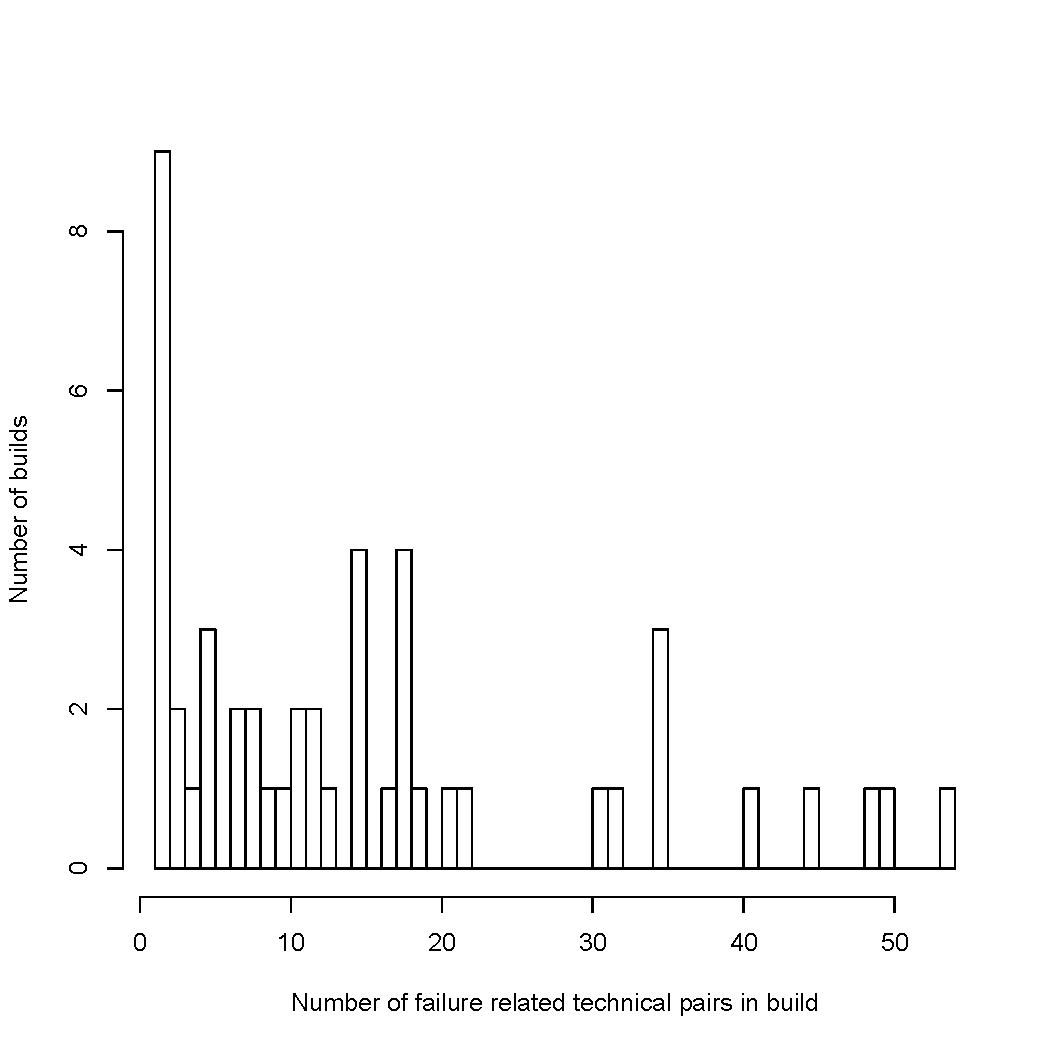
\includegraphics[width=\columnwidth]{figures/builddistribution}
\vspace{-.75cm}
\caption{Histogram plotting how many builds have a certain number of failure-reated technical pairs.}
\label{fig:builddistribution}
\end{figure}

\subsection{Discussion}
% answered the the research question
These results show that there is a strong relationship between certain technical
developer pairs and increased likelihood of a build failure.
% meaning of patterns
Out of the total of 120 technical pairs that increase the likelihood of a
build to fail, only 23 had an existing
corresponding socio-technical pair. Of these, none were statistically
related to build failure. This means that 97 pairs of developers that had a
technical dependency did not communicate with each other and
consequently increased the likelihood of a build failure. Our results not only
corroborate past findings~\cite{cataldo:cscw:2006,cataldo:esem:2008} that socio-technical gaps
have a negative effect in software development. More importantly, they indicate
that the analysis presented in this paper is able to identify the specific
socio-technical gaps, namely the actual developer pairs where the gaps occur
and that increase the likelihood of build failure. 

% contrast of t and st patterns After investigating the pairs closer with respect
% to team allocation, we found that most of the pairs span do not originate from
% the same team.
Although not a goal of this paper, we sought possible explanations for the
socio-technical gaps in this project. A preliminary analysis of developers
membership to teams shows that most
of the technical pairs related to build failure consist of developer belonging to
different teams. Naggappan et al.~\cite{nagappan:icse:2008} found that using the
organizational distance between people predicts failures. They reasoned that this
is due to the lack of awareness what people separated by organizational distance
work on. Although the Jazz team strongly emphasizes communication
regardless of team boundaries, it still seems that organizational distance has
an influence on its communication behavior.

% bridge to regression - confounding variables?
Further, although the analysis of technical pairs in relation to build failures
showed that they have a negative influence on the build result, it does not take
into account possible confounding variables. The question is if there developer pairs still effect the build outcome in the presence of confounding variables, such as number of developers involved in a build, number of work items
related to a build, number of change sets per build, and number of files changed.
We tested this using a logistical regression model including both developer pairs and confounding variables.

Overall the logistic regression confirms the effect of the developer pairs
even in the presence of confounding variables, such as number of files changed
and numbers of developers (AIC of 7006). 
Table~\ref{tab:regression} shows an excerpt from the complete logistical
regression which shows that the twenty pairs previously identified are still
significant under the influence of the four confounding variables. Because we have 2872 developer pairs, space constraints prevent us from reporting the entire regression model. We chose to report on the coefficients for the twenty pairs that we reported in Table~\ref{tab:regression} as well as the coefficients for the four control features.

All features shown in Table~\ref{tab:regression} are significant at the $\alpha=.001$ level (indicated by the p-value and ***).
We checked for all the other technical pairs that were reported significant using the approach described in the previous section and found that they are all significant in the regression model as well.
Moreover, the four control variables of number of developers per build, number
of work items per build, number of change sets per build, and number of files changed per build are also significant.

% explain the coefficient interpretation
% some of the pairs are positive
% some are negative
% extreme magnitude
Since we model failed builds with 0 and successful builds with 1, a negative coefficient means that the feature increases the chances of a failure.
All pairs reported in Table~\ref{tab:regression} and the technical pairs that we identified to be related to build failure have a negative coefficient.
 
% about the control variables
%As shown in Table~\ref{tab:regression} two of the four control features, number of change sets per build and number of developers contributing to a build increase the likelihood of a build succeeding.
%On the other hand number of files changed per build and number of work items per build increase the likelihood of a build failing.

In conclusion, we can answer our second research question with yes: there are
certain technical pairs that are significantly related to build failure, and
this happens even in the presence of possibly confounding variables. 







%\input{regression-analysis}







\section{Practical Implications}
\label{sec:implications}
Our findings have several implications for the design of collaborative systems.
By automating the analyses presented here we can incorporate the knowledge about
developer pairs that tend to be failure related in a real-time recommender
system. Not only do we provide the recommendations that matter to the upcoming
build, we also provide incentives to motivate developers to talk about their
technical dependencies. 

Such a recommender system can use project historical data to
calculate the likelihood that an upcoming build fails given a particular
developer pair that worked on that build without communicating to each other. In
the case of the pair (Adam, Bart) the system may recommend that these
developers should communicate about their technical dependencies, as there
would be a probability
of 91\% of failure of the next build should they not follow the
recommendation. This probability of failure serves as mechanism to
rank importance of a socio-technical gap and more importantly as an
incentive to act upon.

For management, such a recommender system can provide details about the
individual developers in, and properties of, these potentially problematic
developer pairs. Individual developers may be an explanation for the behavior of
the pairs we found in Jazz\texttrademark. This may indicate developers that are
harder to work with or too busy to coordinate appropriately, prompting management
to reorganize teams and workloads. This would minimize the likelihood of a build
to fail, by removing the underlying cause of a pair to be failure related.
Similarly, as another example from our study, most developer pairs
consisted of developers that were part of different teams. In such
situations management may decide to investigate reasons for coordination
problems that include factors such as geographical or functional distance in the project.




\section{Threats To Validity}
\label{sec:threats}
%\todo{rework}
During our study we identified two main threats. 
One threat covers issues that arise from the underlying data we used.
The other threat deals with possible problems from the conceptualization of
constructs in our study.

\subsection{Data}
We performed all our analysis on one set of data, the Jazz\texttrademark\
repository. This limits the generalizability of our findings, due to the fact
that we only made the observations within one project. The  
project size and the project properties -- incorporating open
source practices such as open development and encouraging community involvement
-- make us believe that our findings still hold value.

Furthermore we only investigated three months of the project's lifetime. This
might lead to smaller significance of our results. However, since the three
months are directly before a major release of the project, this dataset contains
the most viable data for our analysis. In those three months a lack of necessary
coordination is the most harmful to the project.

Another threat that is inevitable in studies of software engineers is
the possible lack of recorded communication. This and the possibility of people
coordinating without communicating, such as reading each others source
code~\cite{bolici:stc:2009}, are mitigated in Jazz by its development process.
The Jazz\texttrademark\ team's development process demands that the developers
coordinate using workitem discussion. 


\subsection{Conceptualization}
Our conceptualization of the three edges we use to construct the
socio-technical networks might introduce inaccuracy in our findings.
First, social edges are extracted from workitem discussions. We assumed that
every developer commenting on or subscribed to a work item reads all comments of that
work item. This assumption might not always be correct. By manual inspection of
a selected number of work items, however, we found that developers who
commented on a work item are aware of the other comments, confirming our assumption.

Second, the technical edges are not problematic by themselves, but they are not
complete, since there are more technical relationships between developers that
can be examined. For example, two developers can be connected if one developer
changes someone else's code. This however does not invalidate our findings, it
just suggests that there is room for improvement, which we should address
next.

Third, socio-technical edges on the other hand may suffer from the combination of
social and technical edges. For example, it is not necessarily true that the
discussion of  two developers in a technical dependency is always about their
technical dependency. 
In our study however, since the changes to
source code files we use to extract technical dependencies are attached to workitem discussion, we are
confident that they addressed the changes at least indirectly.



\section{Conclusion}
\label{sec:conclusions}
Our study investigated the relationship between pairs of developers that share
a technical dependency but do not communicate and build failures. We were
motivated by findings in the literature that suggested that high alignment between technical dependencies and actual coordination in a project has a positive effect on task
performance.
%
We hypothesized that a similar relationship may be found in relation to a broader
coordination outcome, i.e. integration outcome, because developers not
coordinating about dependencies in their work might lead to errors remaining in
the code that break the build.

Our case study of coordination in the Jazz project indicates that 
historical project information about socio-technical coordination and software
builds can be used in a model that predicts the quality of upcoming builds. We also found
that the influence of developer pairs with a socio-technical gap on the build
failure was very high. This means that if any one of these pairs was present in a
social network of a build, the build had at least an 74\% chance to fail.
Thus, we add to the literature on failure prediction with a method that
provides actionable knowledge to avoid failures. 

Besides the possible of integrating our findings into a real-time recommender system that indicates the specific developer pairs that should talk about their dependencies, our results add to the research in
collaborative software engineering. Not only do we add to the evidence about
the role of effective communication in the development of high quality
software, but our findings indicate that measures of socio-technical congruence can
serve as a mechanism to identify which inter-personal relationships are
important to avoid breaking software integrations. 
%
We plan to extend this research in a number of directions:

% \begin{description}
\emph{More specific information in socio-technical networks.}
We plan to study socio-technical coordination at a finer level by refining all
three edge types social, technical and socio-technical as well as the
information about developers. For the social edges we plan on identifying who
people are talking to and exactly about what. Technical edges can be refined by examining other source code relations, such as call
graphs, or changes made to others' source code. 
%
To combine social and technical
edges to socio-technical edges we plan to use content analysis techniques on
communication to match it to the appropriate technical edge. We also plan
on also investigating the developers that are part of the social networks more
closely by incorporating developer characteristics, such as experience,
geographical location, role or team allocation.

\emph{Additional edges that indicate emergent coordination.}
In this study we focused on technical pairs and only briefly touched on
socio-technical pairs. In the future we plan to extend this focus to include a
detailed analysis of socio-technical pairs and of those
developer pairs that communicated without sharing a technical dependency, and
which indicate emerging communication in the project, and expertize seeking
behaviors that are important to effective coordination.

\emph{Different types of failures.}
A build fails often because of a single or several failures scattered across several locations
Hence we plan on
investigating single bugs. This additionally enables us to investigate pre-release and post-relase failures separately.
